%General
\documentclass{article}
\usepackage[utf8]{inputenc}
\usepackage{fullpage}

%Symbols
\usepackage{commath}
\usepackage{amsmath}
\usepackage{amssymb}

%Formatting

%%Automata
\usepackage{tikz}
\usetikzlibrary{arrows,automata}

\usepackage{bussproofs}
\usepackage{hyperref}
\usepackage{amsthm}
\usepackage{alltt}
\newtheorem{theorem}{Theorem}[section]
\newtheorem{definition}[theorem]{Definition}
\newtheorem{example}[theorem]{Example}
\hypersetup{colorlinks=true}
\hypersetup{colorlinks=true}
\usepackage{graphicx}
\graphicspath{ {img/} }
\usepackage{caption}

\title{Title}
\date{\today}
\author{Hjort}

\begin{document}
\maketitle

\section*{DFA}
\subsection*{Basic exercises}

\begin{enumerate}
    \item \textbf{Exercise 2.2.4:} Give DFA's accepting the following languages over the alphabet \{0,1\}:

        All these are validated in the Programs folder in this repository, using Erlang

        \begin{enumerate}
            \item The set of all strings ending in $00$.

                $
                \begin{array}{r || c | c}
                        & 0 & 1 \\ \hline \hline
                    \to q_0 & q_1 & q_0 \\
                        q_1 & q_2 & q_0\\
                        *q_2 & q_2 & q_0
                \end{array}
                $

            \item The set of all strings with three consecutive 0's (not necessarliy at the end)

                $ \begin{array}{r||c|c}
                            & 0 & 1 \\ \hline \hline
                    \to q_0 & q_1 & q_0 \\
                    q_1 & q_2 & q_0 \\
                    q_2 & q_3 & q_0 \\
                    *q_3 & q_3 & q_3
                \end{array}
                $

            \item The set of strings with 001 as a substring

                $ \begin{array}{r||c|c}
                            & 0 & 1 \\ \hline \hline
                    \to q_0 & q_1 & q_0 \\
                    q_1 & q_1 & q_2 \\
                    q_2 & q_1 & q_3 \\
                    *q_3 & q_3 & q_3
                \end{array}
                $

        \end{enumerate}

        % 2
    \item
        A language is a regular language iff it is accepted by some finite automata. We thus construct this automata to prove that this is a regular language.

        $ \begin{array}{r||c|c}
            & 0 & 1 \\ \hline \hline
            \to q_0 & q_1 & q_0 \\
            q_1 & q_1 & q_2 \\
            q_2 & q_3 & q_0 \\
            q_3 & q_4 & q_2 \\
            *q_4 & q_1 & q_2
        \end{array}
        $

        \begin{proof}
            (If part) A string ending in 0100 can be in any state when these last digits are encountered. For every state, we follow the arcs labeled 0,1,0,0 in turn and find we always end in $q_4$, which is an accepting state, so the string is accepted.

            (Only if part) A string has been accepted by the DFA. Since it takes a minimum of 4 transitions to get there, the string must be of at least length 4. We can only reach $q_4$ from $q_3$ following a 0, so the last digit must have been 0. We could only get to $q_3$ from $q_2$, following the arc labeled 0, so the string ends in 00. Every arc into $q_2$ is labeled 1, so the string must end in 100. We can get to $q_2$ only from $q_4$, $q_3$ and $q_1$. All these three states only have arcs labeled 0 going int to them, so the string must end in 0100.
        \end{proof}


    \item

        The state diagram for the DFA accpting words containing $bba$ is seen below.

        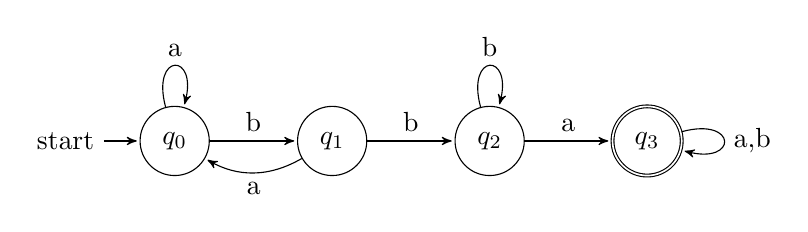
\begin{tikzpicture}[>=stealth',shorten >=1pt,auto,node distance=2cm]
            \node[initial, state]   (q0)    {$q_0$};
            \node[state]            (q1) [right of=q0]    {$q_1$};
            \node[state]            (q2) [right of=q1]    {$q_2$};
            \node[state, accepting] (q3) [right of=q2]    {$q_3$};

            \path[->]
                (q0) edge [loop above]  node {a} (q0)
                     edge   node {b} (q1)
                 (q1) edge  [bend left] node {a} (q0)
                     edge   node {b} (q2)
                (q2) edge   node {a} (q3)
                    edge   [loop above] node {b} (q2)
                (q3) edge  [loop right] node {a,b} (q3);
        \end{tikzpicture}

        The DFA accepting only words without $bba$ as subword must be the words that are not in an accepting state after processing a word with $bba$ as subword, and in an accepting state otherwise. Thus, we simply create an opposite of the DFA above.


        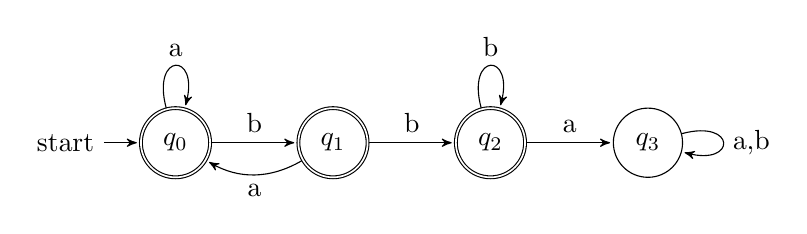
\begin{tikzpicture}[>=stealth',shorten >=1pt,auto,node distance=2cm]
            \node[initial, state, accepting]   (q0)    {$q_0$};
            \node[state, accepting]            (q1) [right of=q0]    {$q_1$};
            \node[state, accepting]            (q2) [right of=q1]    {$q_2$};
            \node[state] (q3) [right of=q2]    {$q_3$};

            \path[->]
                (q0) edge [loop above]  node {a} (q0)
                     edge   node {b} (q1)
                 (q1) edge  [bend left] node {a} (q0)
                     edge   node {b} (q2)
                (q2) edge   node {a} (q3)
                    edge   [loop above] node {b} (q2)
                (q3) edge  [loop right] node {a,b} (q3);
        \end{tikzpicture}

    \item
        \begin{equation*}
            D_1 =
            \begin{array}{r || c | c | c}
                &a  &b  &c \\ \hline \hline
                \to A & B & A & A \\
                B & B & A & C \\
                *C & C & C & C
            \end{array}
        \end{equation*}

        \begin{equation*}
            D_2 =
            \begin{array}{r || c | c | c}
                &a  &b  &c \\ \hline \hline
                \to D & E & D & D \\
                E & E & F & D \\
                *F & F & F & F
            \end{array}
        \end{equation*}

        We then create the DFA $D_3$ which will accept both $ab$ and $ac$ by the product construction.

        \begin{equation*}
        D_3 = (\set{A,B,C} \times \set{D,E,F}, \set{a,b,c}, \delta, AD, \set{C}\times\set{F})
        \end{equation*}

        Where $\delta$ is defined as general in the product rule. We obtain the automata below.

        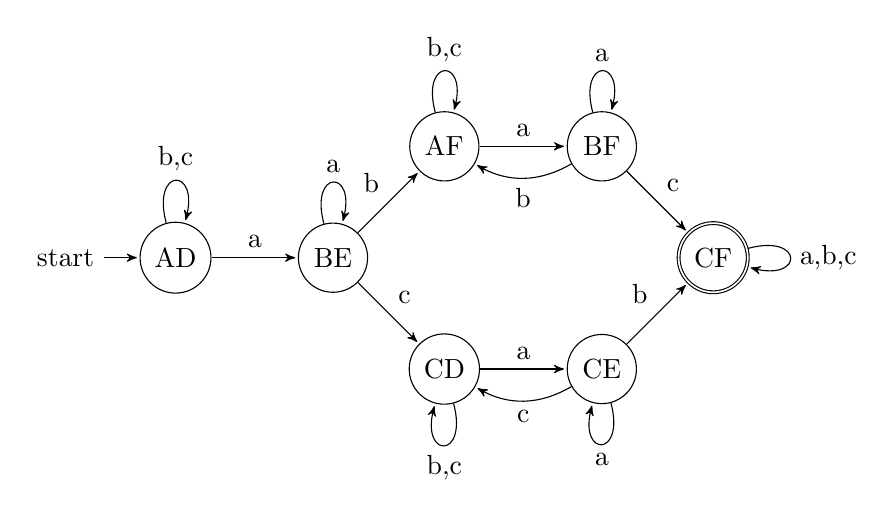
\begin{tikzpicture}[>=stealth',shorten >=1pt,auto,node distance=2cm]
            \node[state, initial] (AD) {AD};
            \node[state] (BE) [right of=AD] {BE};
            \node[state] (AF) [above right of=BE] {AF};
            \node[state] (CD) [below right of=BE] {CD};
            \node[state] (BF) [right of=AF] {BF};
            \node[state] (CE) [right of=CD] {CE};
            \node[state, accepting] (CF) [below right of=BF] {CF};

            \path[->]
                (AD) edge [loop above] node {b,c} (AD)
                    edge node {a} (BE)
                (BE) edge [loop above] node {a} (BE)
                    edge node {b} (AF)
                    edge node {c} (CD)
                (AF) edge [loop above] node {b,c} (AF)
                    edge node {a} (BF)
                (CD) edge [loop below] node {b,c} (CD)
                    edge node {a} (CE)
                (BF) edge [loop above] node {a} (BF)
                    edge [bend left] node {b} (AF)
                    edge node {c} (CF)
                (CE) edge [loop below] node {a} (CE)
                    edge [bend left] node {c} (CD)
                    edge node {b} (CF)
                (CF) edge [loop right] node {a,b,c} (CF)
                   ; 
        \end{tikzpicture}

        For the DFA $D_4$ that accepts $ac$ but not $ab$, we do the product construction of $D_1 \times \overline{D_2}$. The only difference between $D_2$ and its negation is the accepting states, and thus the only difference between $D_3$ and $D_4$ are the accepting states. In $D_4$ the accepting states become $\set{A,B} \times \set{F} = \set{(A,F),(B,F)}$. The automata $D_4$ is shown below.

         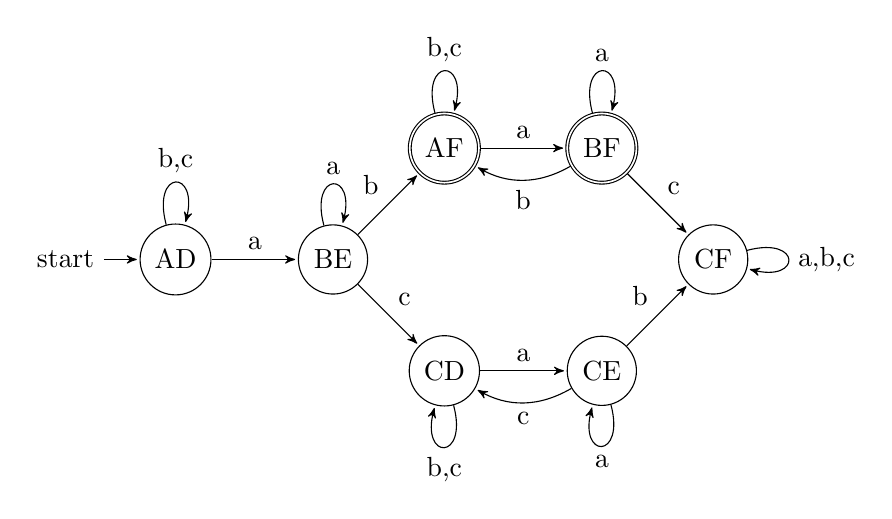
\begin{tikzpicture}[>=stealth',shorten >=1pt,auto,node distance=2cm]
            \node[state, initial] (AD) {AD};
            \node[state] (BE) [right of=AD] {BE};
            \node[state, accepting] (AF) [above right of=BE] {AF};
            \node[state] (CD) [below right of=BE] {CD};
            \node[state,accepting] (BF) [right of=AF] {BF};
            \node[state] (CE) [right of=CD] {CE};
            \node[state] (CF) [below right of=BF] {CF};

            \path[->]
                (AD) edge [loop above] node {b,c} (AD)
                    edge node {a} (BE)
                (BE) edge [loop above] node {a} (BE)
                    edge node {b} (AF)
                    edge node {c} (CD)
                (AF) edge [loop above] node {b,c} (AF)
                    edge node {a} (BF)
                (CD) edge [loop below] node {b,c} (CD)
                    edge node {a} (CE)
                (BF) edge [loop above] node {a} (BF)
                    edge [bend left] node {b} (AF)
                    edge node {c} (CF)
                (CE) edge [loop below] node {a} (CE)
                    edge [bend left] node {c} (CD)
                    edge node {b} (CF)
                (CF) edge [loop right] node {a,b,c} (CF)
                   ; 
        \end{tikzpicture}

    \item
        The language accepted by this DFA is all strings in $\set{0,1}^*$ which have an odd number of 1:s in them.

        Let $w$ be a string in $\set{0,1}^*$. We prove that the above is correct by simple induction on $|w|$.

        We first note that the transition function for this DFA is defined as follows:

        \begin{align*}
            \delta(A,0) = A \\
            \delta(A,1) = B \\
            \delta(B,0) = B \\
            \delta(B,1) = A \\
        \end{align*}

        Let $P(n)$ mean that for strings of length $n$, the only strings accepted are those with an odd number of 1's, and they are all accepted.

        \begin{description}
            \item[Base case]
                $|w|=0 \Rightarrow w = \epsilon$. By definition $\hat{\delta}(q, \epsilon) = q$, so $\hat{\delta}(A,\epsilon) = A$, which is not an accepting state. Since $\epsilon$ contains no 1's, and 0 is an even number, $P(0)$ holds.

            \item[Inductive step]
                Assume $P(n)$. If $|w| = n + 1$ then $w = xa$ where $|x| = n$ and $a \in \set{0,1}$.

                Then $\hat{\delta}(A, w) = \delta(\hat{\delta}(A, x), a)$. Since $P(n)$ holds, we know that $\hat{\delta}(A,x)$ is $A$ if $x$ has an even number of zeroes, ond $B$ if the number is odd.

                We have two cases to consider for $a$: where it is 0, and where it is 1.

                (Case of $a=0$) In this case, we do not transition, but stay in the same state as before. That means $\hat{\delta}(A, w) = \hat{\delta}(A,x)$. Now we also note that $a$ didn't increase the number of 1's, so $w$ contains as many 1's as $x$. Thus, by the inductive hypothesis, we are in A iff $w$ contains an even number of 1's.

                (Case of $a=1$) In this case, we always transition to the other state, and our number of 1's increase by 1. Thus, if $x$ has an even number of 1's, $w$ has an odd number, and vice versa. By the same reasoning as above, if $x$ is accepted then $w$ is not, and vice versa.

                We conclude that $P(n) \Rightarrow P(n+1)$.
                
            \item[Closure]
                Since $P(0) \land (P(n) \Rightarrow P(n+1))$, we conclude $\forall n \in \mathbb{N}. P(n)$.

        \end{description}

\end{enumerate}


\end{document}
